

% LaTeX file for Chapter Exp1



\chapter{Experiment 1: TRAM-DAG (simulation)} \label{ch:exp1}




\section{Motivation}

This experiment demonstrates the application of TRAM-DAGs on a synthetic dataset, using the illustrative DAG previously shown in Figure~\ref{fig:tram_dag}. The objective is to show how TRAM-DAGs can learn causal relationships from observational data, assuming a known DAG. After fitting the model to the joint distribution generated by the underlying causal structure, it is used to sample from observational, interventional, and counterfactual distributions.

The controlled simulation setting allows us to interpret the learned model components in detail and evaluate the model’s ability to recover both linear and nonlinear causal relationships.



% \section{Setup} \label{sec:methods_experiment1}

% To evaluate the TRAM-DAG model, we visualize training performance through the loss curve, interpret the learned transformation components (e.g., intercepts, linear and complex shifts), and assess the model's ability to recover the true data-generating process (DGP). We then sample from the learned model to generate observational and interventional distributions and perform counterfactual queries.


\section{Setup} \label{sec:methods_experiment1}

We visualized the model fitting in terms of the training loss and subsequently showed and interpreted the learned components of the transformation functions, such as intercepts, linear and complex shifts. Finally, we drew samples from the estimated distributions to obtain observational and interventional distributions. We also conducted counterfactual queries on the learned model.

\medskip

\textbf{Data-generating process: } We simulated a dataset with three variables, $X_1$, $X_2$, and $X_3$, following the structure of the DAG and its associated meta-adjacency matrix shown in Figure~\ref{fig:dag_and_matrix}. The matrix describes the functional dependencies between variables, where LS indicates a linear shift and CS a complex shift. Rows represent the source of the effect, and columns the target.


\begin{figure}[H]
\centering
\begin{tikzpicture}[baseline={(current bounding box.center)}]
  \node (img) at (0, 0) {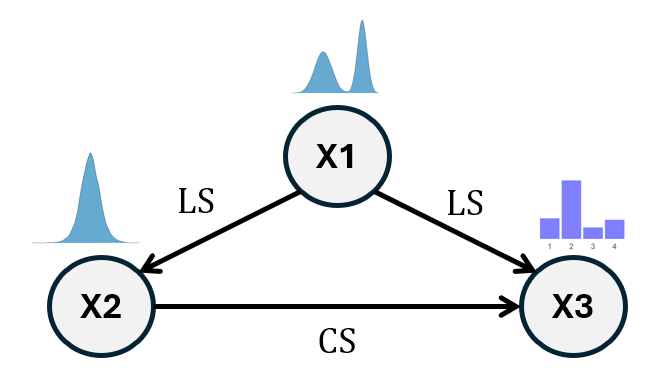
\includegraphics[width=0.28\textwidth]{img/exp1_DAG_MA.png}};
  \node (matrix) at (5, 0) {
    $\mathbf{MA} =
    \begin{bmatrix}
      0 & \text{LS} & \text{LS} \\
      0 & 0  & \text{CS} \\
      0 & 0  & 0
    \end{bmatrix}$
  };
  \draw[->, thick] (img.east) -- (matrix.west);
\end{tikzpicture}
\caption{Causal graph (left) and meta-adjacency matrix (right) for Experiment 1. The transformation function of $X_2$ depends on $X_1$ via a linear shift (LS). The transformation function of $X_3$ depends on $X_1$ via a linear shift (LS) and on $X_2$ via a complex shift (CS).}
\label{fig:dag_and_matrix}
\end{figure}

The variable $X_1$ is continuous and bimodally distributed, and acts as a source node in the DAG, i.e., it is not influenced by any other variable:

\[
X_1 = 
\begin{cases}
\mathcal{N}(0.25,\, 0.1^2) & \text{with probability } 0.5, \\
\mathcal{N}(0.73,\, 0.05^2) & \text{with probability } 0.5
\end{cases}
\]


    
The second variable, $X_2$, is continuous and linearly dependent on $X_1$ on the log-odds scale, with a true coefficient of $\beta_{12} = 2$. Its transformation function is 
\[
h(X_2 \mid X_1) = h_I(X_2) + \beta_{12} X_1,
\]
where the baseline transformation (i.e., intercept) of $X_2$ is $h_I(X_2) = 5 X_2$.

The third variable, $X_3$, is ordinal and depends on both $X_1$ (LS) and $X_2$ (CS). We define the complex shift induced by $X_2$ as $f(X_2) = 0.5 \cdot \exp(X_2)$, and specify the linear shift parameter for $X_1$ as $\beta_{13} = 0.2$. The transformation function for category $k$ of the ordinal variable $X_3$ with 4 levels ($K$) is thus defined by 
\[
h(X_{3,k} \mid X_1, X_2) = \vartheta_k + \beta_{13} X_1 + f(X_2),
\]
with cut-points $\vartheta_k \in \{-2,\, 0.42,\, 1.02\}$ defining the thresholds of the ordinal variable. We generated samples for $X_2$ and $X_3$ as described in Section~\ref{methods:sampling}, by first sampling a latent value from the standard logistic distribution and then determining the corresponding observation using the transformation function.

This simulation allows us to assess whether the TRAM-DAG model can correctly recover the functional forms of the conditional dependencies and the associated parameters (linear and complex).

\medskip

\textbf{Model:} Given the meta-adjacency matrix and the simulated observations, we construct a modular neural network based on the TRAM-DAG framework. The complex shift from $X_2$ to $X_3$ is modeled using a neural network with 4 hidden layers and 2 nodes per layer, as illustrated in Figure~\ref{fig:exp1_CS}. A total of 20,000 samples are generated according to the defined DGP to fit the model. The model is trained for 400 epochs using the Adam optimizer \citep{kingma2015} with a learning rate of 0.005.


% include the figure for CS

\begin{figure}[H]
\centering
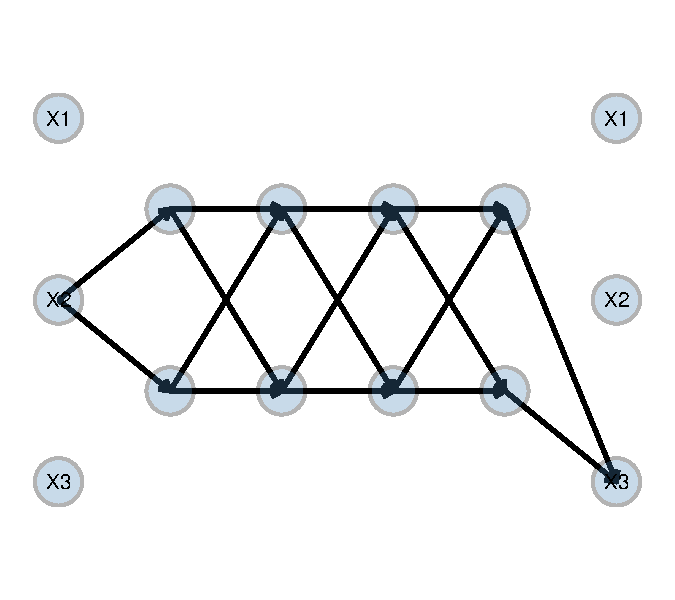
\includegraphics[width=0.5\linewidth]{img/exp1_CS.pdf}
\caption{Neural network architecture for the complex shift on $X_3$ from $X_2$. The complex shift is modeled by a neural network with 4 hidden layers of shape (2, 2, 2, 2), using non-linear activation functions (sigmoid).}
\label{fig:exp1_CS}
\end{figure}




\textbf{Model evaluation: } We compare the estimated intercepts, learned coefficients, and the complex shift to the true values used in the DGP. We also compare the sampled observational and interventional distributions to the true distributions. For the counterfactual queries, we show the estimated counterfactual values for $X_2$ under an intervention on $X_1$ at a specific value, and compare these to the true counterfactual outcomes.




\section{Results}



We evaluate whether TRAM-DAGs can recover the structural equations and distributions used in the data-generating process described in Section~\ref{sec:methods_experiment1}. Below, we present the training process and inspect the estimated parameters, distributions, and counterfactual predictions.

Figure \ref{fig:exp1_loss_parameters} shows the loss and the estimated parameters for the linear shifts over epochs during training. The loss was minimized during training and the estimated parameters $\beta_{12}$ and $\beta_{13}$ converged to the true values used in the DGP. The linear shift parameters are the interpretable part of the model (log-odds ratios). From the fitted model, we generated samples from the observational distribution, as shown in Figure \ref{fig:exp1_observational_distribution}. The TRAM-DAG can recover the observational distribution as its samples align with the data that was used to fit the model. Then we drew samples from the interventional distribution, where $X_2 = 1$ is fixed, as shown in Figure \ref{fig:exp1_interventional_distribution}. Fixing $X_2$ leads to a distributional change in $X_3$, which was also captured by the model. The TRAM-DAG learns the linear shifts ($\beta_{12}$, $\beta_{13}$) and the complex shift $f(X_2)$, which are shown in Figure \ref{fig:exp1_shifts}. Figure~\ref{fig:exp1_intercepts} presents the intercepts learned for each of the nodes. For comparison, we added the estimated intercept functions from the Continuous Outcome Logistic Regression (Colr() function from the \texttt{tram} package \citep{hothorn2018}) for $X_1$ and $X_2$, and the true values used in the DGP for the ordinal variable $X_3$ (three cut-points for the four levels). Since the transformation functions for $X_1$ and $X_2$ contain no complex terms, they match the default form used in Colr(). Finally, Figure~\ref{fig:exp1_counterfactuals} shows the counterfactuals for $X_2$ estimated by the TRAM-DAG for varying values of $X_1$. The counterfactuals are the predicted values of $X_2$ had $X_1$ taken other values instead of the initially observed one. 

\begin{figure}[htbp]
\centering
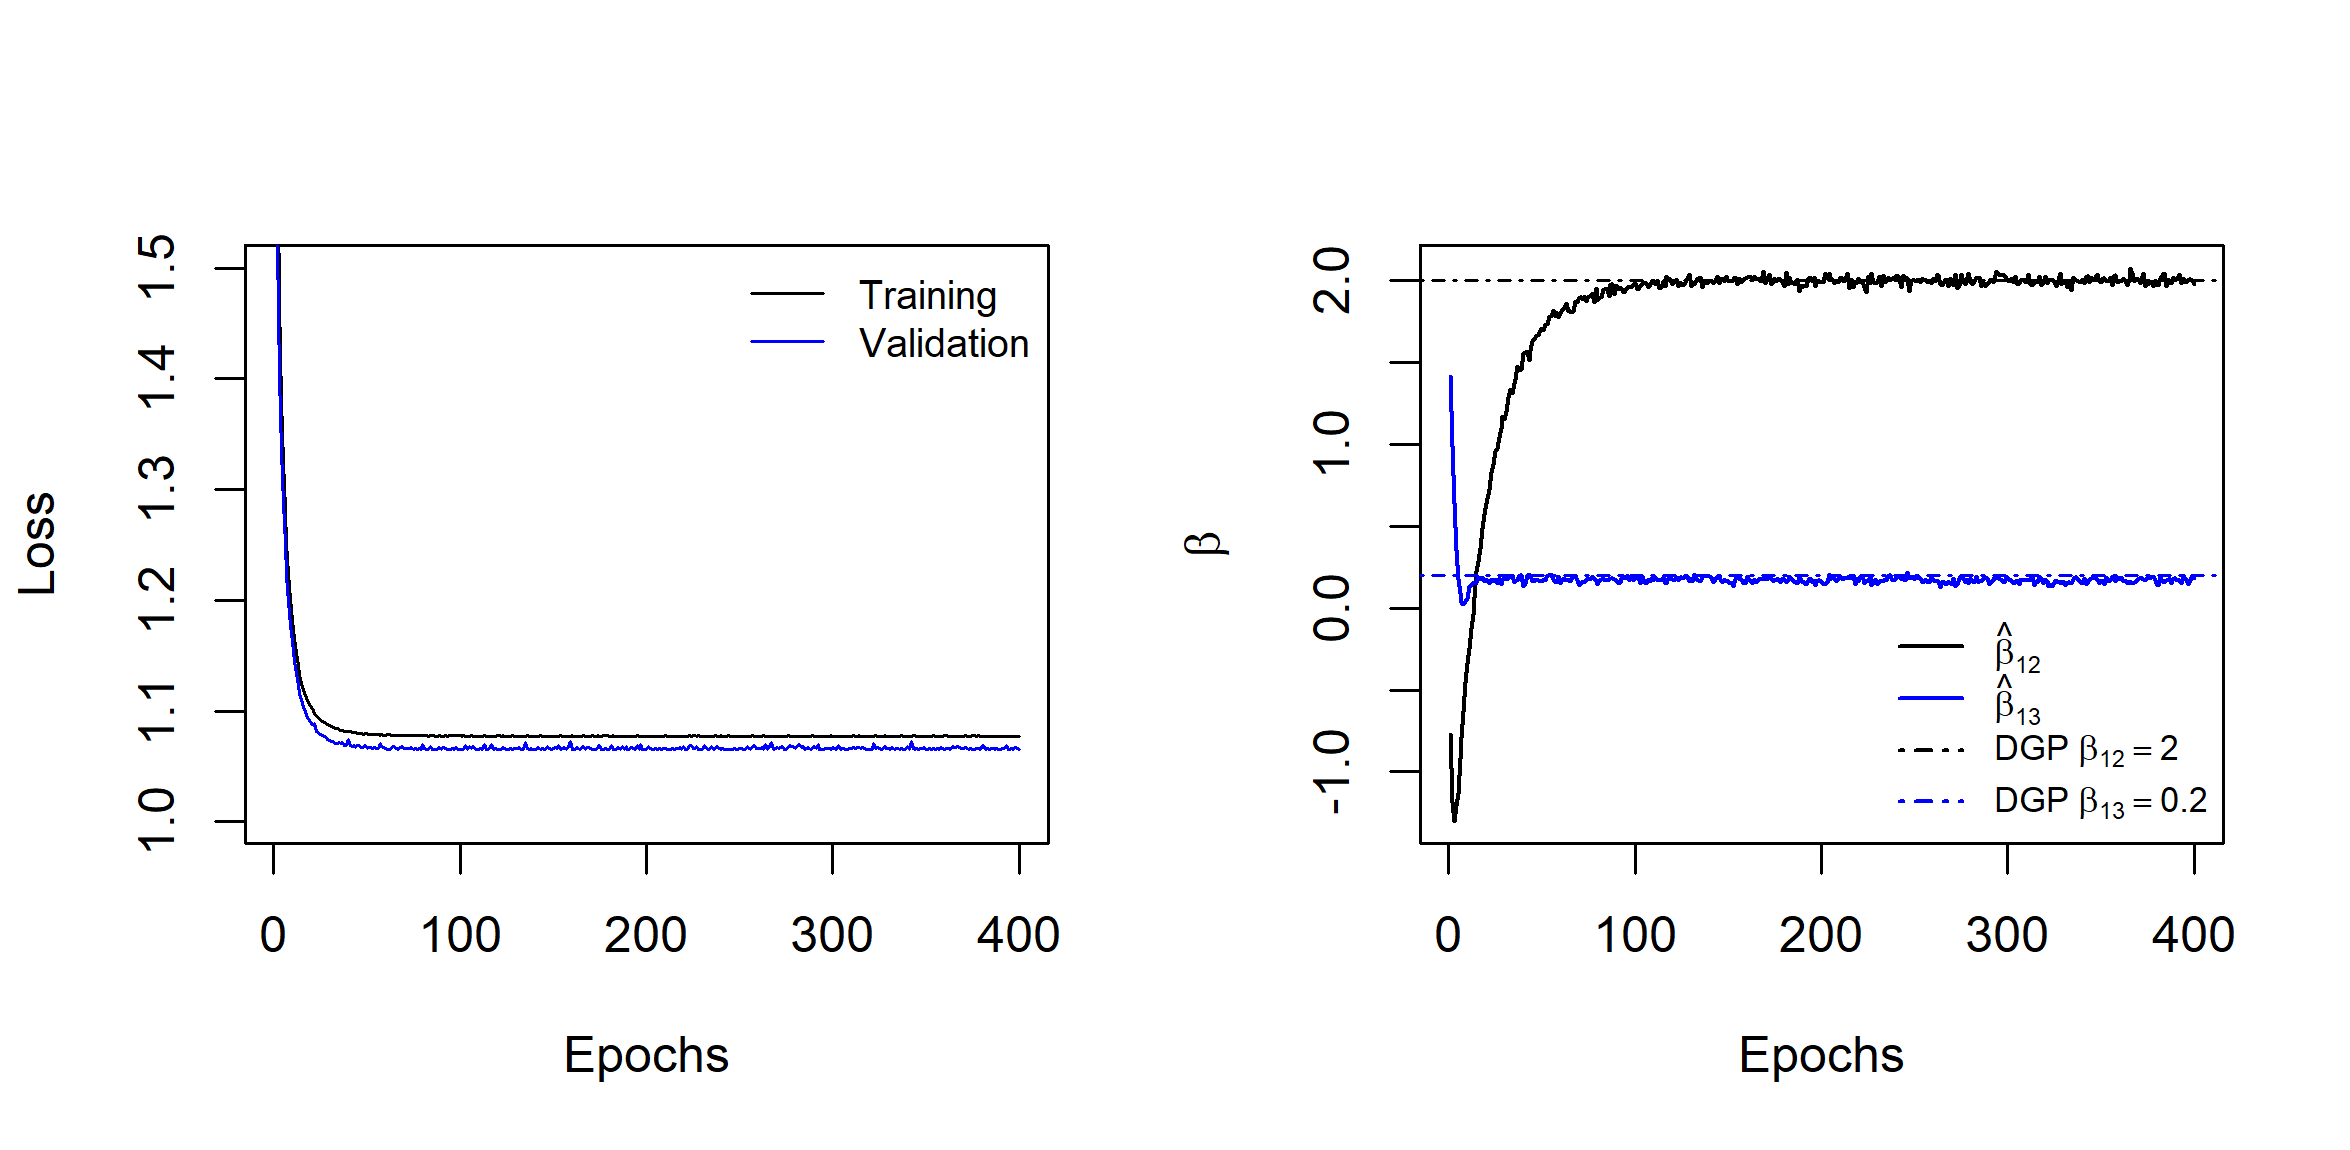
\includegraphics[width=0.9\textwidth]{img/exp1_loss_parameters.png}
\caption{TRAM-DAG model fitting over 400 epochs for Experiment 1. Left: loss functions on the training and validation sets; Right: estimated parameters (betas) for the linear shift components over epochs. The estimates converge to the true values used in the DGP.}
\label{fig:exp1_loss_parameters}
\end{figure}



\begin{figure}[htbp]
\centering
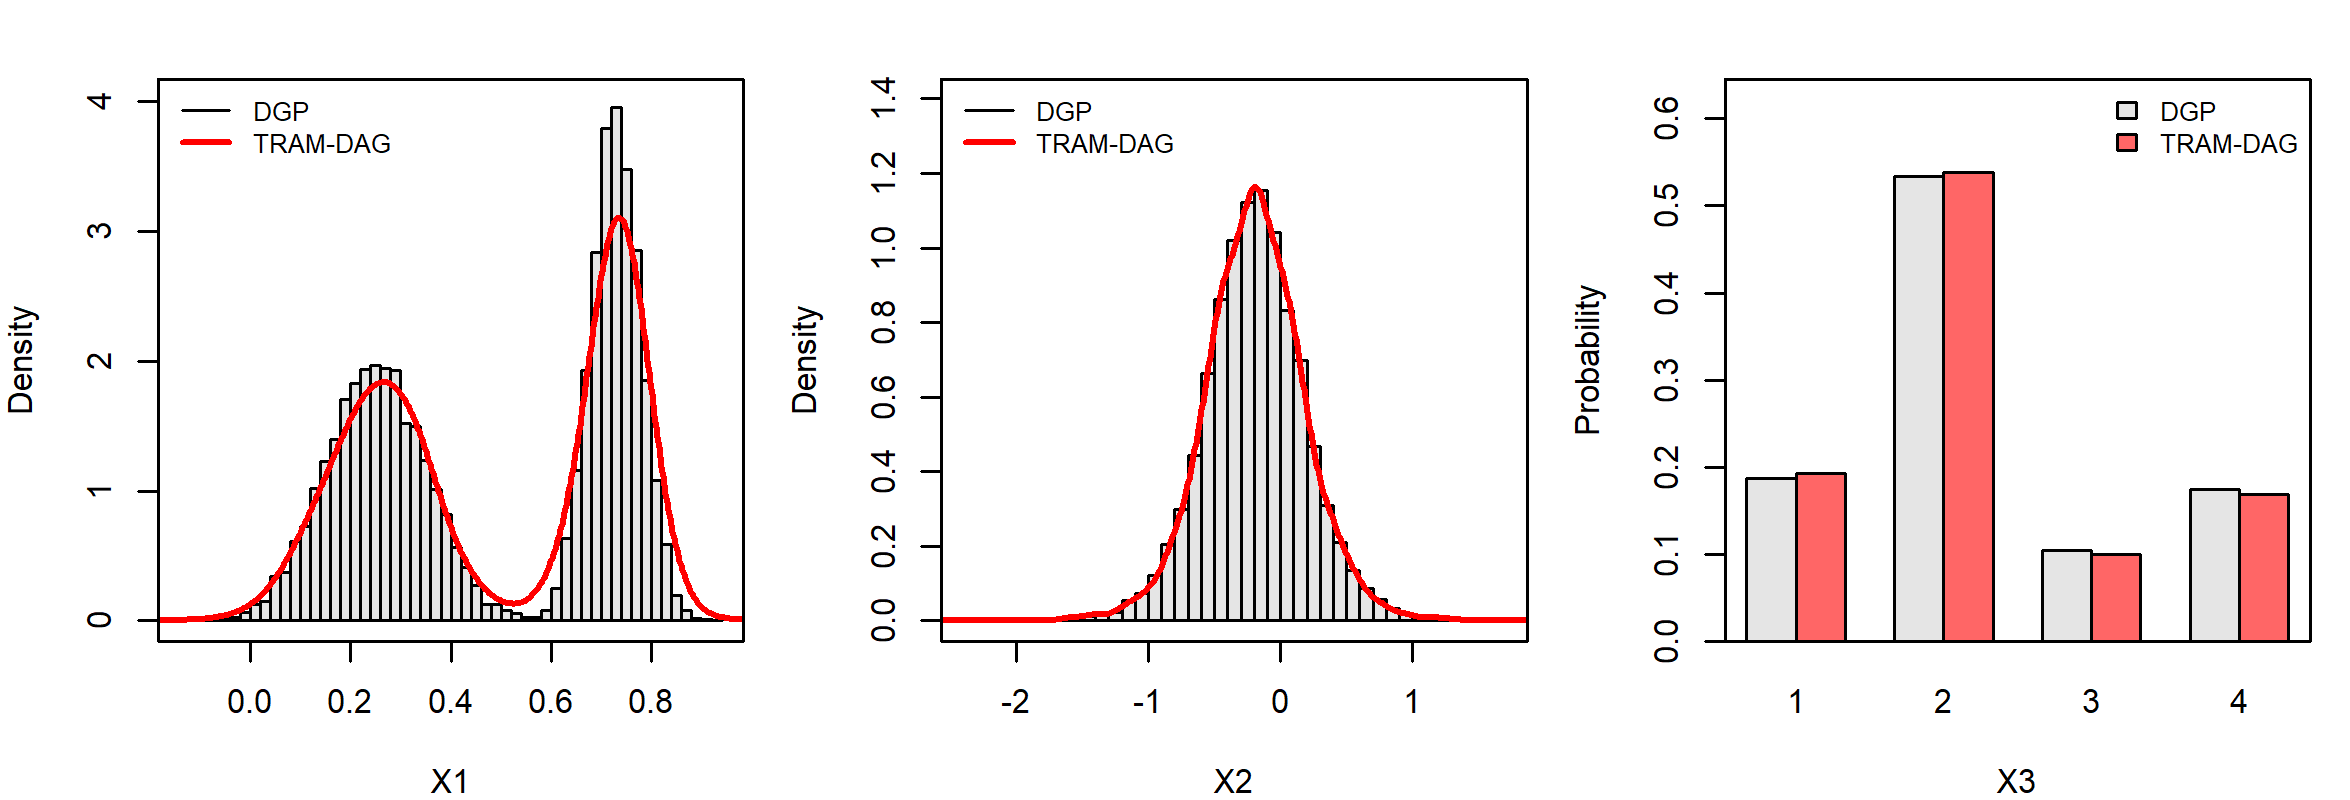
\includegraphics[width=0.9\textwidth]{img/exp1_observational_distribution.png}
\caption{Samples generated by the TRAM-DAG from the learned observational distribution, compared to the true observations from the DGP.}
\label{fig:exp1_observational_distribution}
\end{figure}




\begin{figure}[htbp]
\centering
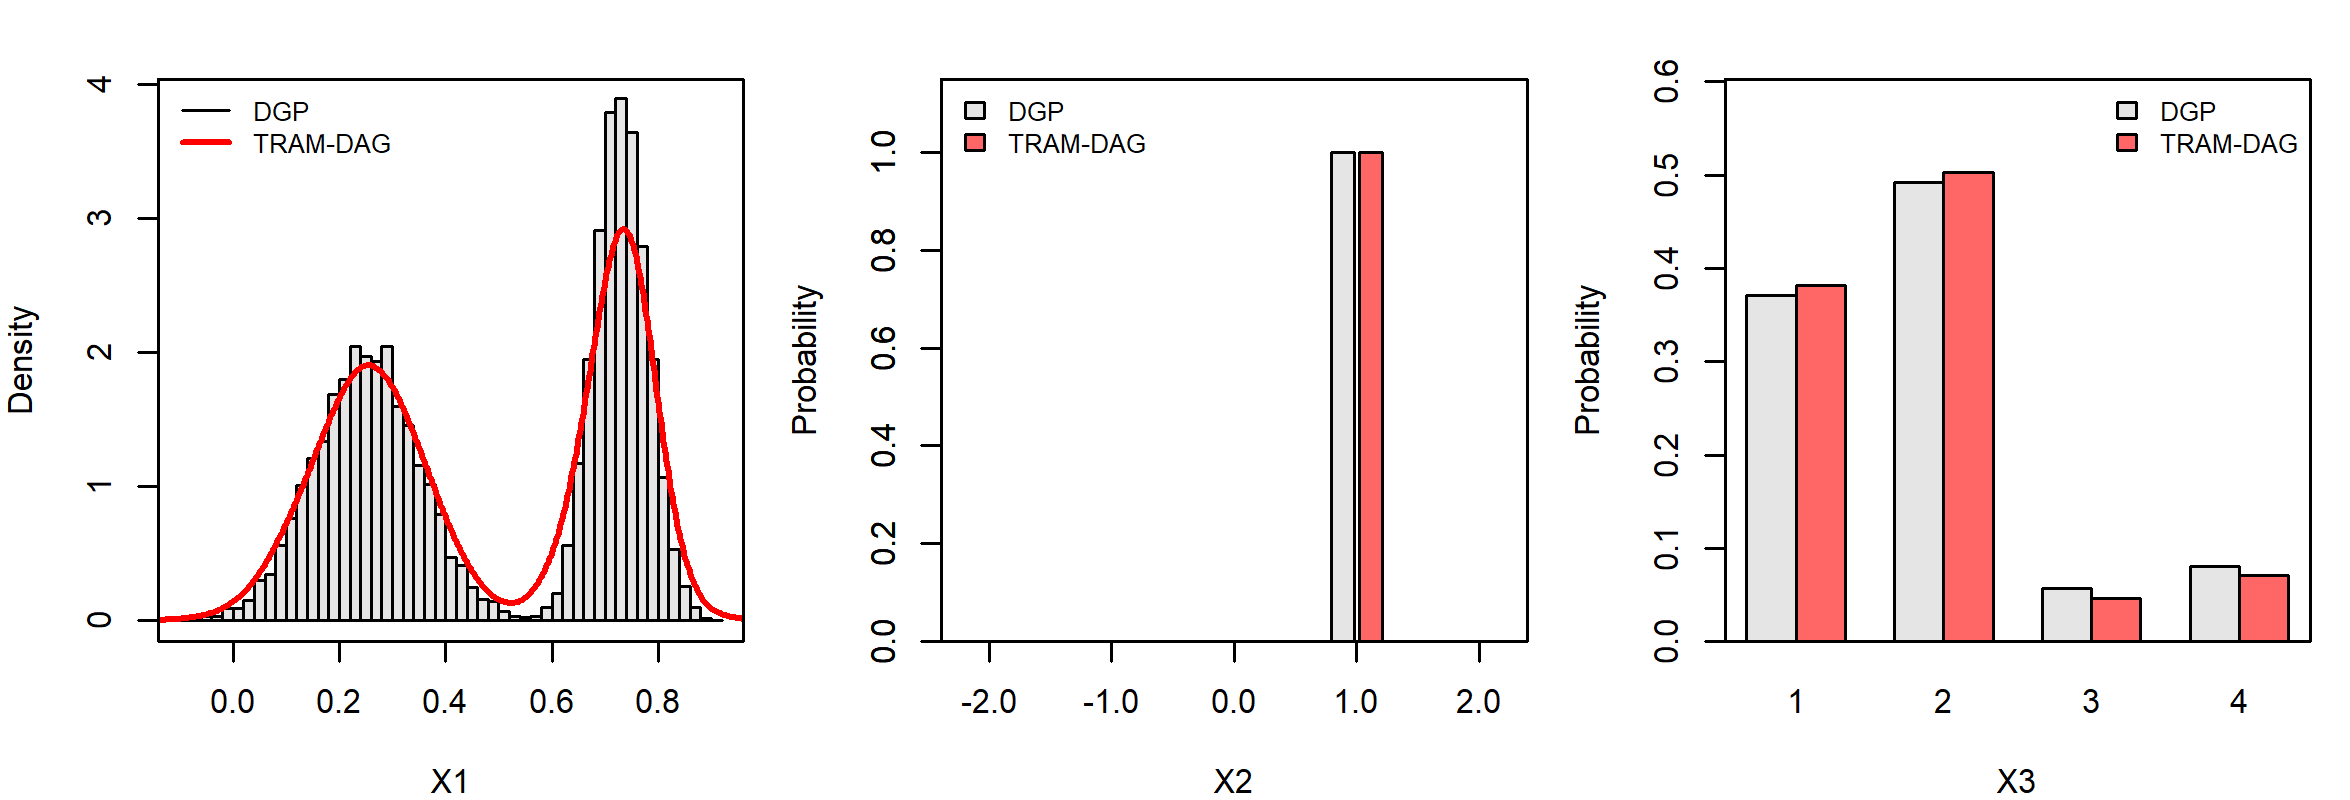
\includegraphics[width=0.9\textwidth]{img/exp1_interventional_distribution.png}
\caption{Samples generated by the TRAM-DAG compared to the true observations from the interventional distribution of the DGP, where $X_2 = 1$ is fixed. According to the DAG, this intervention induces a distributional change in $X_3$.}
\label{fig:exp1_interventional_distribution}
\end{figure}



\begin{figure}[htbp]
\centering
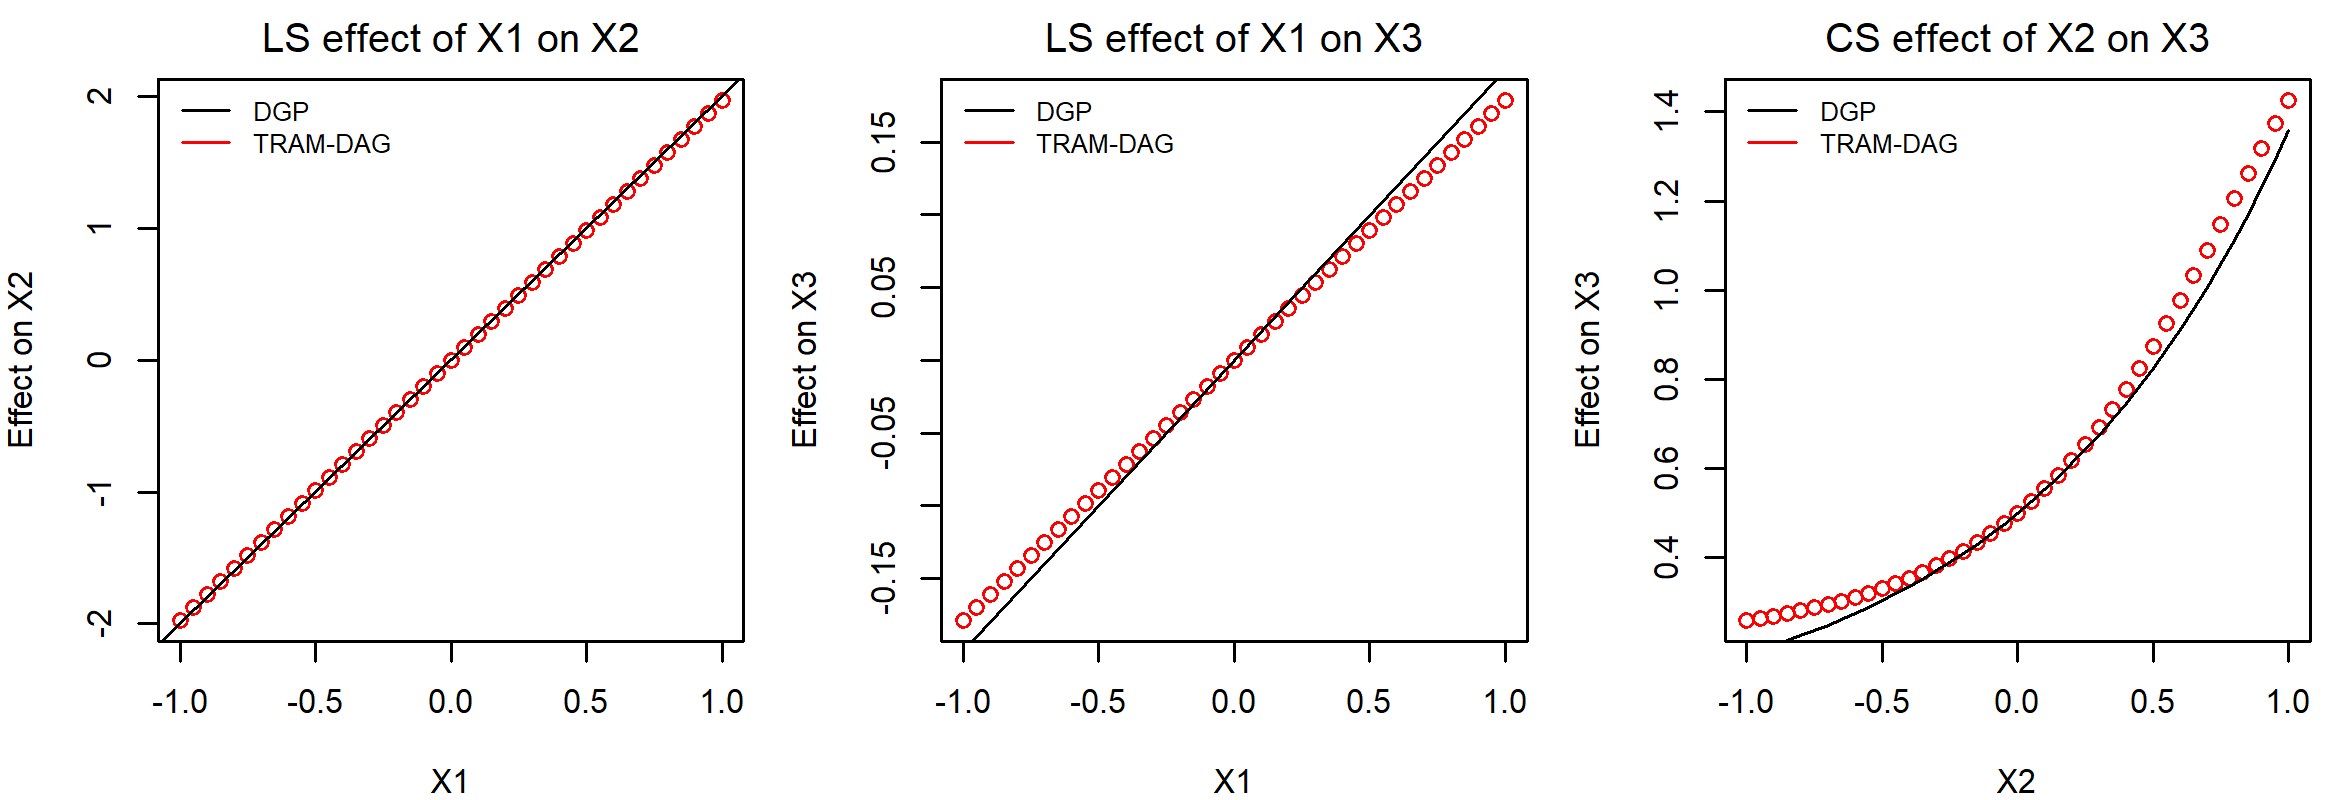
\includegraphics[width=0.9\textwidth]{img/exp1_LS_CS.png}
\caption{Linear and complex shifts learned by the TRAM-DAG. Left: LS($X_1$) on $X_2$; Middle: LS($X_1$) on $X_3$; Right: CS($X_2$) on $X_3$. For visualization, we subtracted $\delta_0 = \text{CS}(0) - f(0)$ from the estimated complex shift CS($X_2$) to align it with the true shift function $f(X_2)$ from the DGP.}
\label{fig:exp1_shifts}
\end{figure}



\begin{figure}[htbp]
\centering
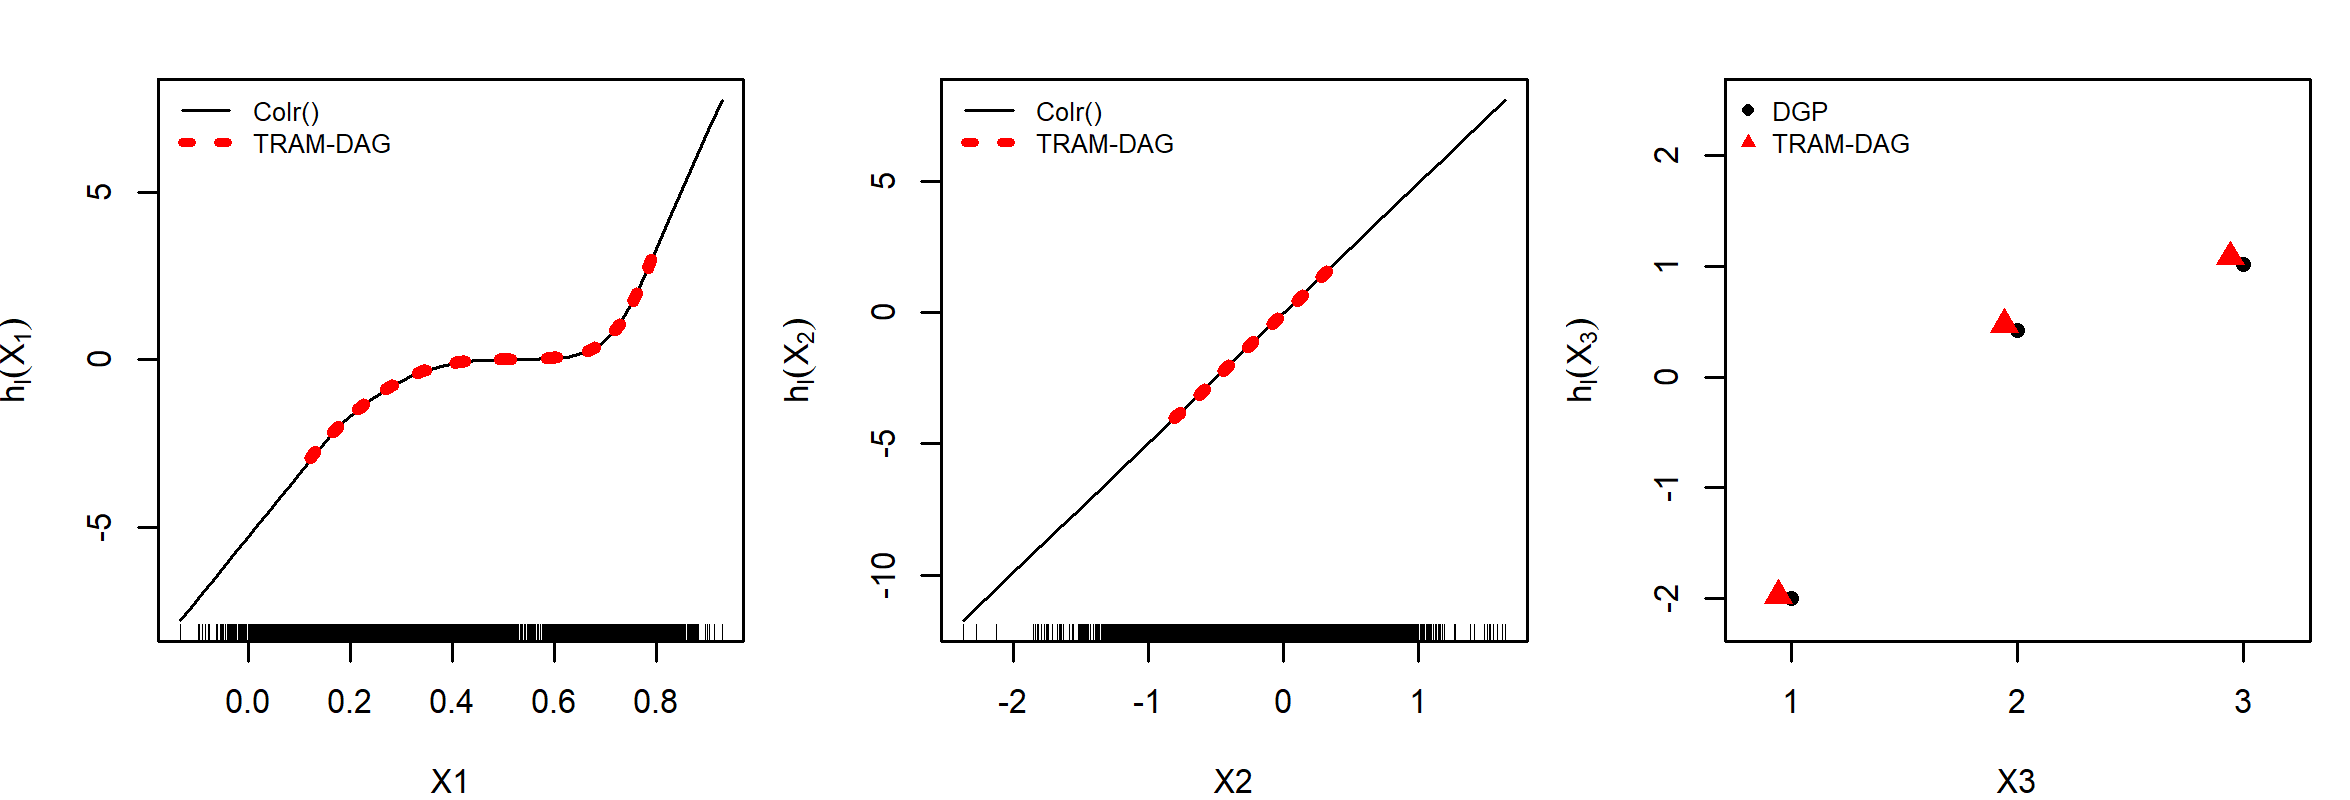
\includegraphics[width=0.9\textwidth]{img/exp1_baseline_trafo.png}
\caption{Intercepts learned for each of the nodes, along with the estimates from the \texttt{Colr()} function for the continuous variables and the true values from the DGP for the ordinal variable $X_3$. Left: Smooth baseline transformation function for continuous $X_1$; Middle: Smooth baseline transformation function for continuous $X_2$; Right: Cut-points as the baseline transformation function for ordinal $X_3$. For the last plot, we added $\delta_0 = \text{CS}(0) - f(0)$ to the estimated cut-offs to make them comparable to the true parameters from the DGP.}
\label{fig:exp1_intercepts}
\end{figure}




\begin{figure}[htbp]
\centering
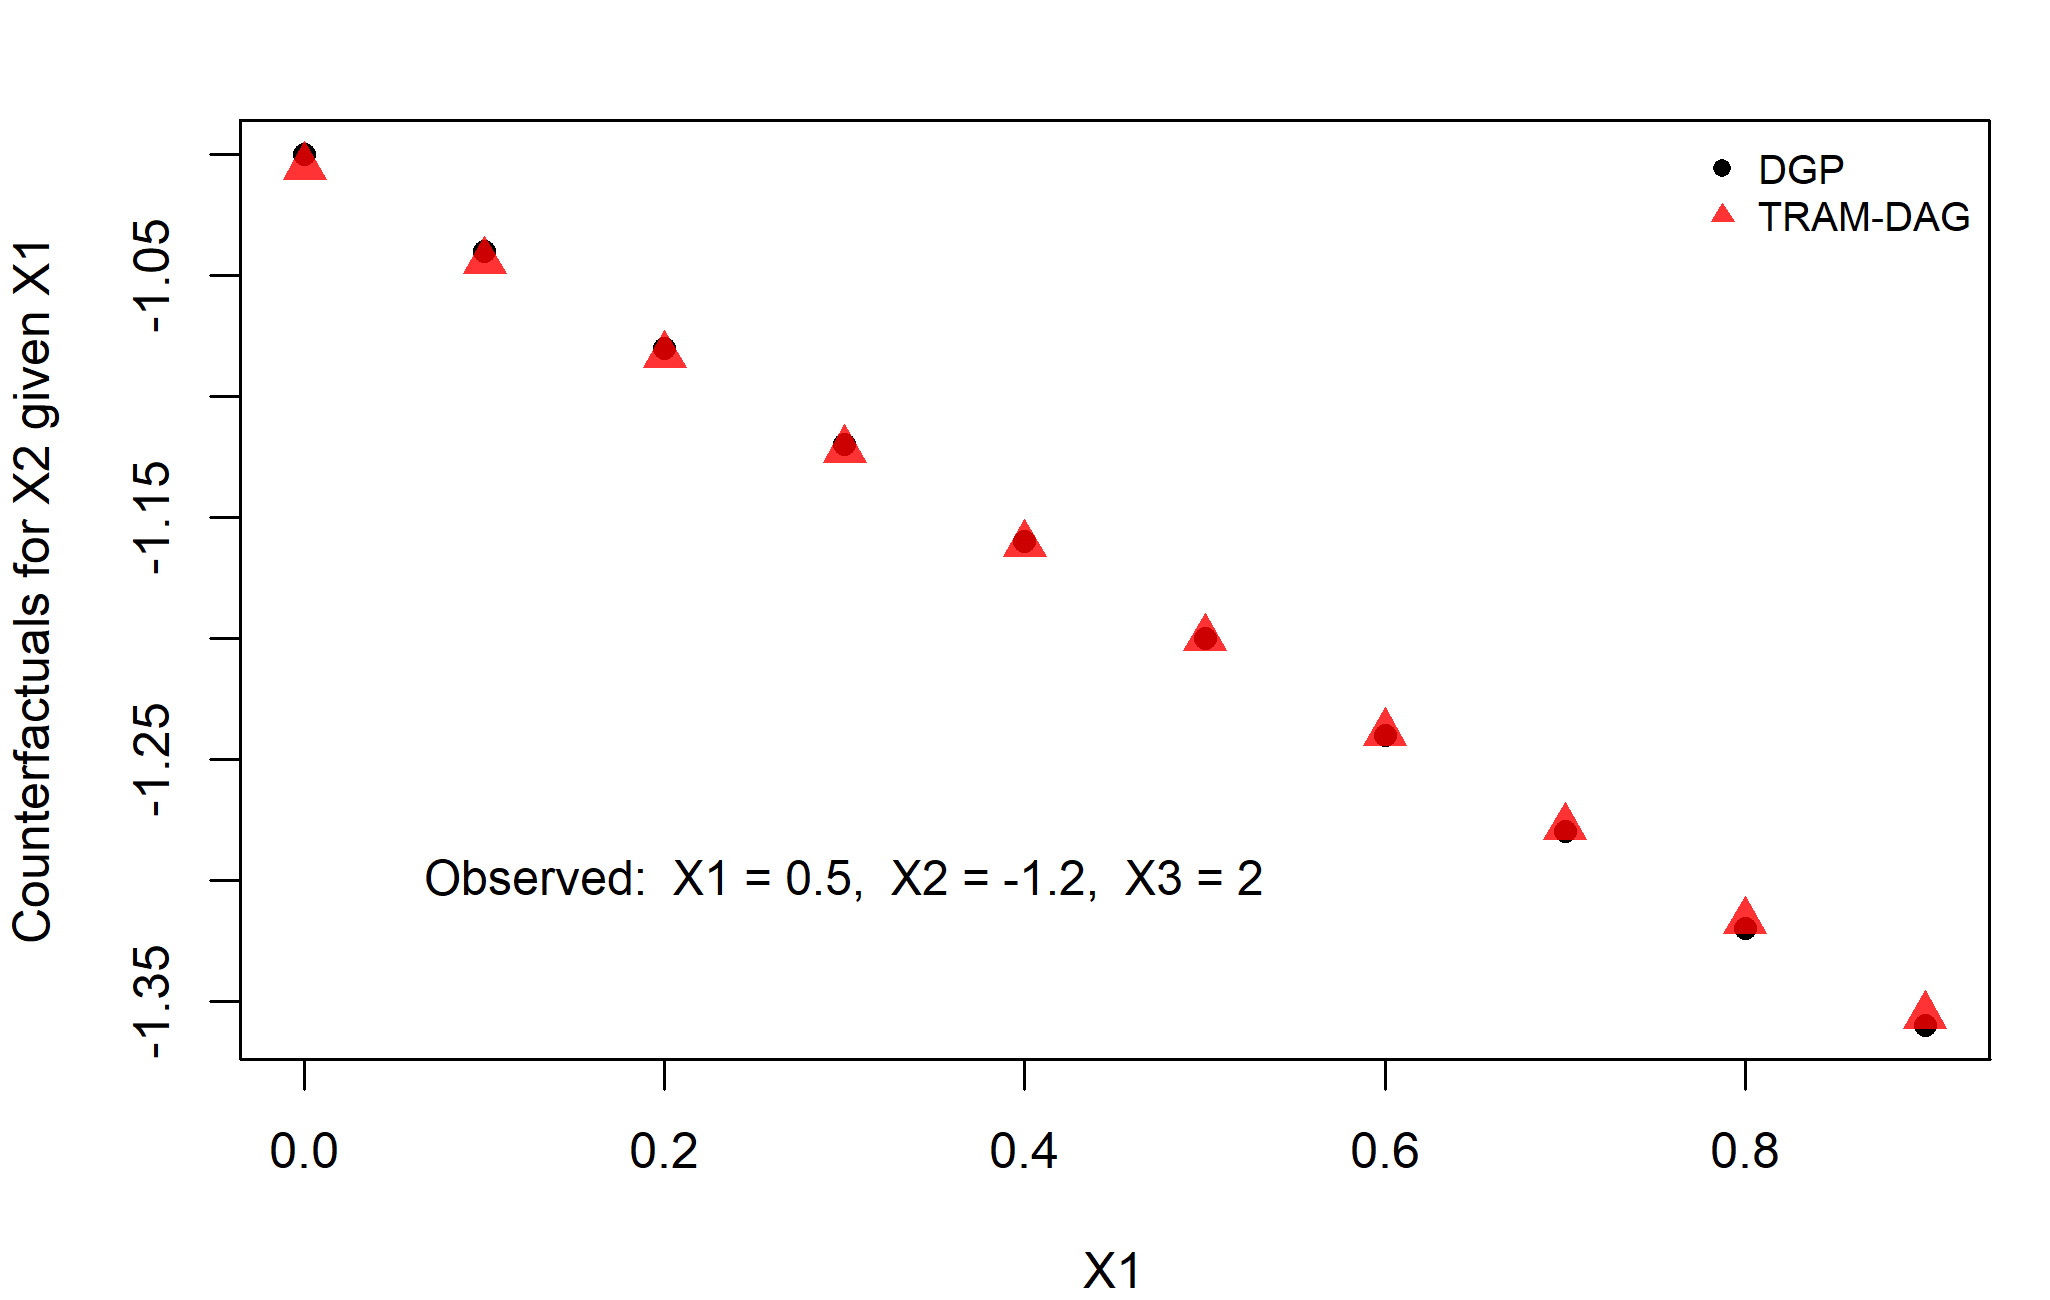
\includegraphics[width=0.9\textwidth]{img/exp1_counterfactuals.png}

\caption{Counterfactuals for $X_2$ estimated with the TRAM-DAG for varying values of $X_1$. We assumed the observed values $X_1 = 0.5$, $X_2 = -1.2$, and $X_3 = 2$, and determined the counterfactual values of $X_2$ had $X_1$ taken different values instead of the actually observed one. This illustrates how the model estimates alternative outcomes under hypothetical interventions on $X_1$.}
\label{fig:exp1_counterfactuals}
\end{figure}



% enforce that starts after all floats have been displayed
\FloatBarrier

\section{Discussion}

The results show that the TRAM-DAG framework can accurately recover the underlying causal relationships from data, including both linear and nonlinear (complex) relationships. This enabled the model to generate observational and interventional distributions that closely matched the true ones, and to produce valid counterfactual predictions.

This experiment provides a simple proof of concept for the flexibility and generative capability of TRAM-DAGs. By incorporating both interpretable (e.g., linear shifts) and flexible (e.g., complex shift) components, the model is able to capture a range of causal mechanisms -- provided that the true DAG is known and data is generated accordingly.


% \section{Discussion}
% 
% 
% The results demonstrate that the TRAM-DAG framework can learn the true parameters and both linear and complex shifts from the data, enabling it to act as a generative model for predicting interventions and counterfactuals. It successfully reproduced observational and interventional distributions and predicted correct counterfactual outcomes.
% 
% This experiment serves as a small proof of concept that TRAM-DAGs can be specified flexibly, with both interpretable and complex components, to capture causal relationships of varying complexity when the true DAG is known and the data is generated accordingly.



